% TODO several class diagrams shown here seem to be pixel graphics and should be replaced by vectorized ones

\subsection{Recap on Object-Orientation and Design Patterns}

\begin{frame}{Recap: Object Orientation}
	\begin{mycolumns}[height=50mm]
		\begin{definition}{Key Concepts}
			\begin{itemize}
				\item \textbf{Encapsulation}:\\abstraction and information hiding
				\item \textbf{Composition}:\\nested objects
				\item \textbf{Message Passing}:\\delegating responsibility
				\item \textbf{Distribution of Responsibility}:\\separation of concerns
				\item \textbf{Inheritance}:\\conceptual hierarchy, polymorphism, reuse
			\end{itemize}
		\end{definition}
	\mynextcolumn
		\pic[width=\linewidth]{oo-concepts-illustration} % TODO what illustrates which concept? why is square not a rectangle or rectangle not a square?
	\end{mycolumns}
\end{frame}

\begin{frame}{Recap: Design Patterns\ \mytitlesource{\gof}}
	\begin{mycolumns}[widths={60}]
		\begin{definition}{Design patterns \deutsch{Entwurfsmuster}}
			\begin{itemize}
				\item Document common solutions to concrete yet frequently occurring design problems
				\item Suggest a concrete implementation for a specific object-oriented programming problem
			\end{itemize}
		\end{definition}	
		\begin{note}{Design Patterns for Variability}
			Many Gang of Four (GoF) design patterns for designing software around stable abstractions and interchangeable (i.e., variable) parts, e.g.
			\begin{itemize}
				\item Template Method
				\item Abstract Factory
				\item Decorator
			\end{itemize}
		\end{note}
	\mynextcolumn
		\picborder{\pic[width=\linewidth]{gof}}
	\end{mycolumns}
\end{frame}

\subsection{Template Method Pattern}
\begin{frame}{\myframetitle}
	\begin{mycolumns}[widths={40}]
		\begin{definition}{Template Method \mysource{\gof\mypages{325--330}}}
			\begin{itemize}
				\item {\bf Intent:} \mycite{Define the overall structure of an algorithm, while allowing subclasses to refine, or redefine, certain steps.}
				\item {\bf Motivation:}  Avoid code replication by implementing the general workflow of an algorithm once, while allowing for necessary variations.
				\item {\bf Idea:} A template method defines the skeleton of an algorithm. Concrete methods override the hook methods.
			\end{itemize}
		\end{definition}
	\mynextcolumn
		\pic[width=\linewidth]{templatemethod}
	\end{mycolumns}
\end{frame}

\subsection{Abstract Factory Pattern}
\begin{frame}{\myframetitle}
	\begin{mycolumns}[widths={40}]
		\begin{definition}{Abstract Factory \mysource{\gof\mypages{87--95}}}
			\begin{itemize}
				\item {\bf Intent:} \mycite{Provide an interface for creating families of related or dependent objects without specifying their concrete classes.}
				\item {\bf Motivation:} Avoid case distinctions when creating objects of certain kind, consistently create objects of a particular kind.
				\item {\bf Idea:} Create classes for the consistent creation of objects.
			\end{itemize}
		\end{definition}
	\mynextcolumn
		\pic[width=\linewidth]{abstractfactory}
	\end{mycolumns}
\end{frame}

\subsection{Decorator Pattern}
\begin{frame}{\myframetitle}
	\begin{mycolumns}[widths={40}]
		\begin{definition}{Decorator \mysource{\gof\mypages{175--184}}}
			\begin{itemize}
				\item {\bf Intent:} \mycite{Attach additional responsibilities to an object dynamically. Decorators provide a flexible alternative to subclassing for extending functionality.}
				\item {\bf Motivation:} Avoid explosion of static classes when combining all additional behaviors with all applicable classes.
				\item {\bf Idea:} Create decorators and components with the same interface, whereas decorators forward behavior whenever feasible.
			\end{itemize}
		\end{definition}
	\mynextcolumn
		\pic[width=\linewidth]{decorator}
	\end{mycolumns}
\end{frame}

\subsection{Trade-Offs and Limitations}

\begin{frame}{Object-Oriented Design of our Graph Library}
	\begin{mycolumns}[widths={40}]
		\pic[width=\linewidth]{graphlib-oo-node-edge}
	\mynextcolumn
		\pic[width=\linewidth]{graphlib-oo-graph}
	\end{mycolumns}
\end{frame}

\begin{frame}[fragile]{Instantiation Through Template Method Pattern}
	\small
	\begin{mycolumns}[widths={45}]
\begin{codetight}{}
class Graph {
	...
	Edge add(Node n, Node m) {
		Edge e = createEdge();
		nv.add(n); nv.add(m); ev.add(e);
		return e;
	}
	// hook method (with default implementation)
	Edge createEdge(Node n, Node m) {
		return new Edge(n, m);
	}
}
\end{codetight}
\begin{codetight}{}
@class WeightedGraph extends Graph {
	...
	// override hook method
	Edge createEdge(Node n, Node m) {
		Edge e = new WeightedEdge(n, m);
		e.weight = new Weight();
		return e;
	}
}@
\end{codetight}
	\mynextcolumn
		\centering\pic[width=.7\linewidth]{graphlib-oo-node-edge}
	\end{mycolumns}
\end{frame}

\begin{frame}[fragile]{Instantiation Through Abstract Factory Pattern}
	\begin{mycolumns}[b]
\begin{codetight}{}
class Graph {
	EdgeFactory edgeFactory;
	...
	Graph(EdgeFactory edgeFactory) {
		this.edgeFactory = edgeFactory;
	}
	Edge add(Node n, Node m) {
		Edge e = edgeFactory.createEdge(n, m);
		nodes.add(n); nodes.add(m); edges.add(e);
		return e;
	}
}
\end{codetight}
\begin{codetight}{}
class EdgeFactory {
	Edge createEdge(Node a, Node b) {
		return new Edge(a, b);
	}
}
\end{codetight}
	\mynextcolumn
		\centering\pic[width=.75\linewidth]{graphlib-oo-node-edge}	
\begin{codetight}{}
@class WeightedEdgeFactory extends EdgeFactory {
	Edge createEdge(Node a, Node b) {
		Edge e = new WeightedEdge(n, m);
		e.weight = new Weight();
		return e;
	}
}@
\end{codetight}
	\end{mycolumns}
\end{frame}

\begin{frame}{Feature Combinations?}
	\centering\pic[width=.5\linewidth]{graphlib-oo-diamond}
\end{frame}

\begin{frame}{Diamond Problem}
	\begin{mycolumns}
		\begin{note}{Multiple Inheritance}
			\begin{itemize}
				\item most object-oriented programming languages do not support multiple inheritance (or only provide workarounds)
				\item critical: how to handle name clashes
			\end{itemize}
			% TODO add quote on multiple inheritance?
			% Multiple Inheritance is like a parachute. You don't often need it, but when you do, you really need it. Grady Booch? this one does not really fit here
		\end{note}
	\mynextcolumn
		\pic[width=\linewidth]{graphlib-oo-diamond-commented}
	\end{mycolumns}
\end{frame}

\begin{frame}{Static Modeling of Feature Combinations}
	\begin{mycolumns}[columns=3,widths={10,80},animation=none]
	\mynextcolumn
		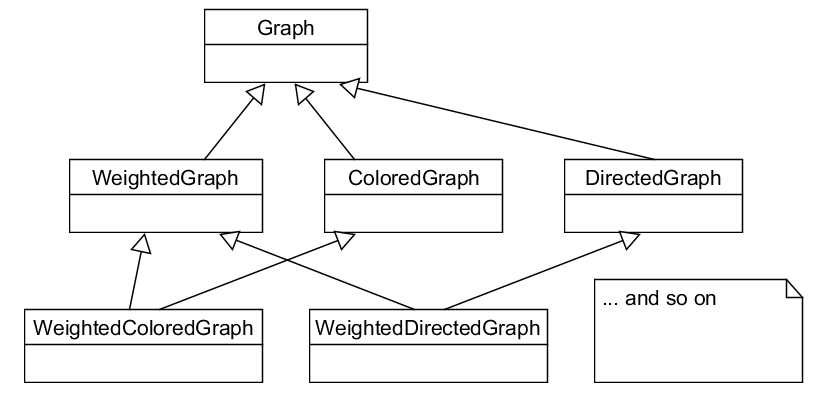
\includegraphics[width=\linewidth]{graphlib-oo-combinatorial}
		\mynote{}{
			Even if multiple inheritance is supported, statically combining features through inheritance is tedious (or infeasible).
		}
	\mynextcolumn
	\end{mycolumns}
\end{frame}

\begin{frame}[fragile]{Decorator Pattern as a Solution?} % TODO motivation too short
	\begin{mycolumns}[widths={52}]
		\small
\begin{codetight}{}
abstract class GraphDecorator implements IGraph {
	IGraph graph;
	GraphDecorator(IGraph graph) {
		this.graph = graph;
	}
}
\end{codetight}
\begin{codetight}{}
@class WeightedGraph extends GraphDecorator {
	WeightedGraph(IGraph graph) {
		super(graph);
	}
	Edge add(Node n, Node m) {
		WeightedEdge e = (WeightedEdge) graph.add(n, m);
		e.weight = new Weight();
		return e;
	}
	...
}@
\end{codetight} % TODO old slides had a further example. add it?
	\mynextcolumn
		\pic[width=\linewidth]{graphlib-oo-decorator}
	\end{mycolumns}
	\small
\begin{codetight}{Example Usage}
IGraph graph = @new WeightedGraph(@~new ColoredGraph(~new Graph(@new WeightedEdgeFactory()@)~)~@)@;
\end{codetight}
\end{frame}

\begin{frame}{Delegation Instead of Inheritance}
	\begin{mycolumns}[widths={55}]
		\begin{note}{Discussion}
			Extensions (i.e., features) can be combined dynamically, but \ldots
			\begin{itemize}
				\item must be independent of each other
				\item cannot add public methods
				\item runtime overhead due to indirections
				\item several physical objects are forming a conceptual one (e.g., problems with object identity)
			\end{itemize}
		\end{note}
	\mynextcolumn
		\pic[width=\linewidth]{graphlib-oo-decorator}
	\end{mycolumns}
\end{frame}
